\section{Experiment}
\label{sec:experiment}
\shuqing{Many parts in this section are much more likely to lie in implementation, introducing how \tool works. Doesn't look like experiment.}

%\shuqing{Experiment for devices and case study needed.}
To evaluate the effectiveness of \tool, we conducted experiments in the three modes introduced in the Section~\ref{sec:badusb} on devices with USB Type-C capabilities.

\textit{Setup.} Our implementation contains a USB Type-C hub with HDMI and USB port, a Raspberry Pi 4B with a Wi-Fi chip onboard, a video capture card adapting HDMI signal to USB camera, and a normal power bank with dual outputs.
\shuqing{Figures of our power bank.}
The power bank is used to supply the Raspberry Pi 4B and charge the victim's devices.
The USB Type-C hub adapts USB Type-C to a HDMI port and USB ports, which is used to connect HID devices and transmit video stream from victim's devices to HDMI port. 
The video stream will be captured by the Raspberry Pi 4B through the video capture card.
Note that in the following experiments, we chose different types of devices, i.e., smartphones, PCs and iPads, to conduct experiments in different modes to validate the usability and effectiveness of \tool.

\subsection{Scripting mode}

We used \textit{Lenovo Xiaoxin Pro 13 2020}, a PC in Windows 10 with two USB Type-C interfaces as target device while conducting the experiment in scripting mode. 
In this experiment, \tool disguised itself as a normal keyboard.
Similar as BadUSB~\cite{badusb}, \tool injected keystrokes at a high speed to start a terminal (cmd.exe) by hotkey, and executed the malicious scripts in it.
Through executing scripts, \tool could implant viruses, worms, backdoors, etc. into hosts, which would make the victim's devices under significant risk.
However, scripting mode can only be used on devices which terminal is available, limiting its capabilities to PC.

\subsection{Remote control mode}
We chose \textit{iPad Pro (3rd generation)}, a tablet in iOS 14.3 with a USB Type-C interface, as the target device in this experiment.
Besides performing as normal HID devices as conventional BadUSB~\cite{badusb}, \tool could transmit real-time video streaming of screen from the target device to the attacker through WiFi or GSM.
\tool captured video from USB Type-C Hub's HDMI output via a video capture card, streamed video with \textit{FFmpeg}, a video processing utility and uploaded video stream to the attacker's device.
With a real-time video stream as an indicator, attackers can precisely control the position of mouse movements and clicks, controlling the iPad to open applications, peek at the victim's photos, etc.

Remote control mode is ideal for the attackers to control the victim's devices and grab all information shown on the victim's devices. 
However, it needs user consent for the first time and requires high power consumption to encode video streams and stable network connections.
In the real world, high power consumption will increase the possibilities of being noticed by the victim, and stable network connections is hardly guaranteed.


\subsection{Privacy extraction mode}
We chose \textit{HUAWEI P30}, a smartphone in EMUI 9.1 (Android 9.0 based) with a USB Type-C interface, as the target device in this experiment.
As remote control mode, \tool captured video from the victim's device and use \textit{opencv} to identify valuable information from video stream. 
When the victim viewed text or photos with text, \tool used the techniques of optical character recognition (OCR) to extract text from corresponding video frames. \yechang{hyperlink to OCR?}\shuqing{I think we don't need to explain OCR nor put a reference link.}
For example, we extracted the victim's name, photo, address, and ID number when victim is viewing his/her photos of his/her ID card or passport documents,
We also extracted the victim's payment information when victim is using bank apps or payment apps.
Besides, \tool used \textit{opencv} to detect and decode QR codes or barcodes shown on the victim's device, which is expected to extract payment code information in the payment apps.
Here is an example of extracting payment code with opencv library in listing. \shuqing{Need to be modified.}\shuqing{Do we plan to add this?}

Privacy extraction mode only extracts valuable information for attackers (or highly sensitive information for victims), which is more efficient  than remote control mode.

%\begin{lstlisting}[caption={python script for extracting payment code of victim},label=lst2:qr]
%import cv2, qrcode,requests
%import pyzbar.pyzbar as pyzbar
%def decodeDisplay(video):
%    gray = cv2.cvtColor(video, cv2.COLOR_BGR2GRAY)
%    barcodes = pyzbar.decode(gray)
%    for barcode in barcodes:
%        barData = barcode.data.decode()
%        barType = barcode.type
%        requests.post('<server of attacker>',
%            data={
%                'data': barData,
%                'type': barType
%            }
%        )
%if __name__ == '__main__':
%    cam = cv2.VideoCapture(0)
%    while True:
%        ret, frame = cam.read()
%        decodeDisplay(frame)
%        if cv2.waitKey(5) == 27:
%            break
%    cam.release()
%    cv2.destroyAllWindows()
%\end{lstlisting}


\subsection{Case study}

\subsubsection{Background}

We conducted a case study with sharing power bank and QR code payment as technical background.

\textbf{Sharing Power Bank}. 
Sharing power bank provides users with short-term rental of power banks. 
The provider deploys power bank stations in the city, while the users can rent a power bank from any of the power bank station, charge their device on the trip, return the rented power bank to another station, and pay the rent online.

As an example, Brick is such a power bank sharing service provider from Sweden. 
As Brick's website states, \textit{Brick prevents your electronics from running out of battery with power banks (Bricks) that you can easily rent \& return at our many stations in Stockholm, Gothenburg, Malmö and the rest of Sweden and even Europe.}. \yechang{citation needed}
\shuqing{I think we should paraphrase instead of using the descriptions on the website directly. Just to explain \textbf{what we need}.}

\begin{figure}[t]
	\centering
	\includegraphics[width=.4 \linewidth]{./Figs/Brick_station.png}
	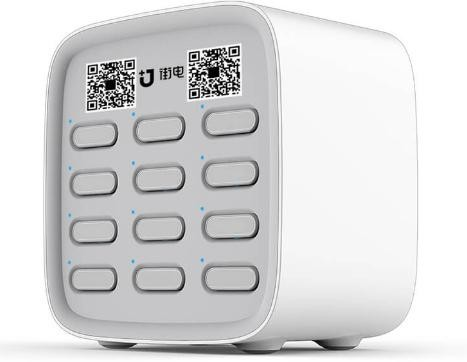
\includegraphics[width=.4 \linewidth]{./Figs/jiedian.jpg}
	\caption{Two power banks station products}\shuqing{Photos that we took.}
	\label{fig:PBS_products}
\end{figure}

\yechang{add hyperlink or reference to Brick's website or Brick App on App Store/Google Play.}

\yechang{Add more examples of power bank sharing to show that it is widely used?}
\shuqing{May use statistics (instead of concrete examples) to explain it.}

Though it provides convenience to users, it also brings security issues. 
We noticed that most of the power bank stations do not check the integrity of power banks during the rental process, and users are hardly cautious to check the power banks when connecting their devices to them. 
The attackers are able to modify their rented power banks, return it to a power bank station as normal.
Then the subsequent users will unknowingly connect to such malicious power banks, which endangers the financial security and data security of users.


\textbf{QR Code Payment}. 
QR code payment is a method of paying bills, typically performed as the following steps:
\ding{182} The payer opens the payment application on his/her mobile device, and present his/her payment QR code to the payee. 
This QR code is encoded with a globally unique ID to identify the payer's account. 
\ding{183} The payee scan the payment QR code presented by the payer. 
By presenting this QR code, the payer authorizes proceeding with the payment.
\ding{184} An order generated by this scan is sent to the payment service provider. 
Then the payment service provider requests the payer to confirm the transaction.
\ding{185} After confirmation, the payment service provider proceed with this transaction and return the payment result to both the payee and the payer.
\shuqing{I think this paragraph can be shorter. No need to explain so many details.}

\begin{figure}[t]
	\centering
	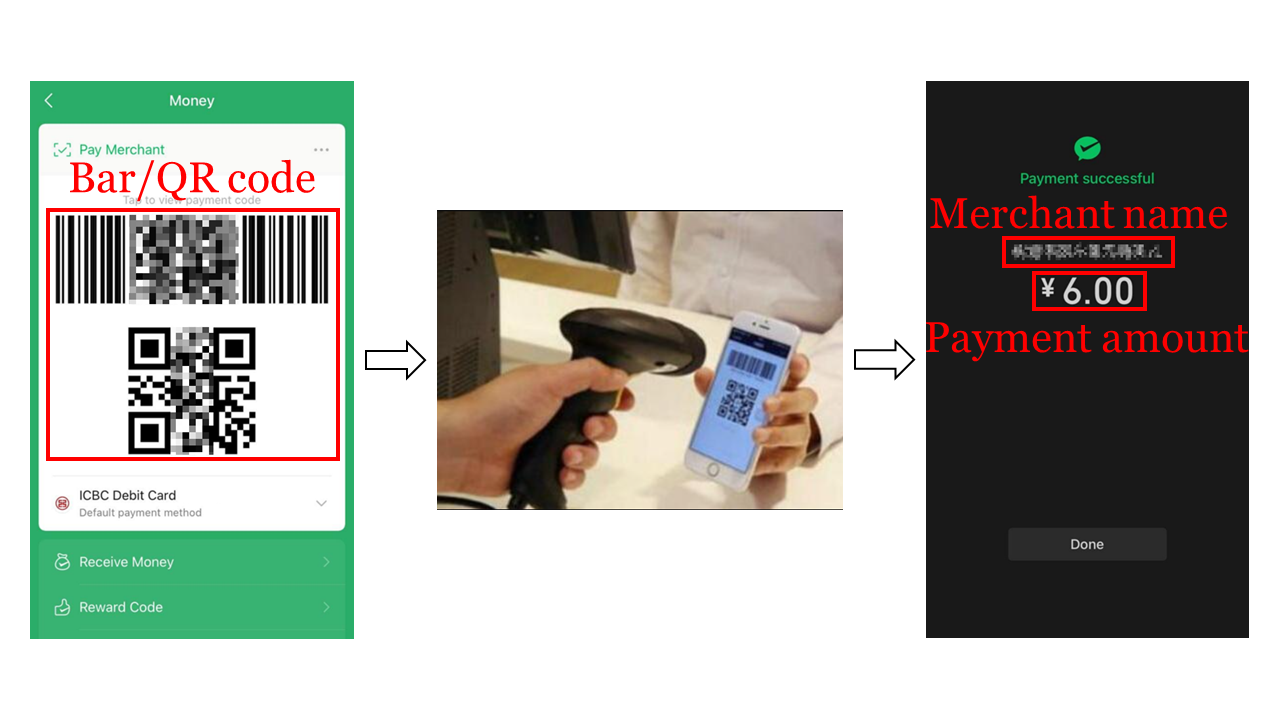
\includegraphics[width=\linewidth]{./Figs/qr_code_payment.png}
	\caption{Bar/QR code payment procedure}
	\label{fig:qr_payment_procedure}
\end{figure}


In the real-world scenario, some payment service providers provide special rules for micropayment purchases. 
A micropayment is pre-determined by the payment service provider with thresholds in the user agreement. 
For example, WeChat Pay~\cite{Wechat-pay} regards payments less than CNY \textyen 1000 as micropayments. 
Different from a typical payment procedure, when micropayments are made, confirmations can be applied automatically without requiring the payer to take further actions, which is often encouraged by the payment service provider.
The payment QR code is associated with the payer's account. 
If a victim's payment code is leaked to the attackers, they can use the that payment code to proceed payments. 
Furthermore, the attackers can use several micropayments to steal money from the victim's account, leaving the victim unconscious. 
\shuqing{Introduce something about QR code refreshing (fast).}
In summary, the payment QR code is highly sensitive on users' devices.

\subsubsection{Attack Scenario}

Note that \tool only exposes a type-c cable (from USB Type-C hub).
It charges the attacker's device through this cable, which has no difference from ordinary power banks. 
Considering users' vigilance and high similarity between \tool and normal power banks, the attackers can put the modified power banks (e.g., \tool) in a power bank station.
Subsequent users may unconsciously connect their devices to \tool.
Like many outdoor mobile phone usage scenarios\shuqing{Any reference? How frequent the payment code is used?}, the victim may complete payment with showing payment code. 
Then the attackers can extract and use the victim's payment code to make another payment unknown to the victim.
\shuqing{This paragraph is duplicate with some previous paragraphs. We can make the previous introduction abut attack scenario really brief, and mainly introduce it here.}

\shuqing{Background is longer than real user study.}
In order to validate the usability of \tool, we conducted a user study in privacy extraction mode. 
\shuqing{10 volunteers.}
We invited 6 volunteers to take part in, who are unconscious of the experiment details.
Volunteers took turns to operate their phones for half an hour while \tool is connected, which they considered as a normal power bank.
After the study, we introduced to them about our attack, checked the screen recordings together, and get the permission to study the information in recorded videos.
\shuqing{Do we need to mention that agreement the conference required here?}
Subject to efficiency reasons, we asked them to use phones just like when they use the shared power bank outside.
\shuqing{What does it mean?}


\subsubsection{Result}

After collecting the videos, we analyzed the videos both automatically and manually. 
During the automatic analysis, we used scripts to perform OCR recognition for each frame in the recorded video and stored all of the OCR results in a database.
At last, there are 38329 pieces of data collected among 6 volunteers.
\shuqing{The data may need to be updated.} 
With these results, we could learn what content the victim was browsing.
Additionally, some keywords such as \textit{account, username and password} often appear with users' input data because they are often used as labels of input boxes.
Such keywords are more likely to lead us to discover user-specific data.
For example, when we searched with \textit{account} as keyword, victim's accounts can be found in the database, as shown in the Table~\ref{tab:ocr_keyword_example}.
\shuqing{Statistics.}
The frame number is the position of this frame in the recorded video, which indicates a target for manual analysis for further data extraction.

\begin{table*}[t]
	\centering
	\begin{tabular}{|l|l|l|l|}
		\hline
		Keyword  & Text                                                                                                                          & Name                           & Frame Number \\ \hline
		username & X 8B cas.******.edu.cn Username: 117***18 Password:                                                                           & \textless{}user1\textgreater{} & 385          \\ \hline
		username & Login Weibo Login with SMS and verification code ...... +86 151****4587 Get verification code Login with username \& password & \textless{}user5\textgreater{} & 1947         \\ \hline
		username & QQ 14*****50| Login with phone number New user registration 2345678 9 0                                                       & \textless{}user3\textgreater{} & 4308         \\ \hline
		username & connect to *** username h*****l Save account information Open VPN.....                                                        & \textless{}user6\textgreater{} & 7925         \\ \hline
		+86      & Login with phone number ...... +86 186****2483 |                                                                              & \textless{}user1\textgreater{} & 313          \\ \hline
	\end{tabular}
	\caption{Example of searching OCR results with some keywords}
	\label{tab:ocr_keyword_example}
\end{table*}


In the manual analysis, we replayed the recorded video and extracted sensitive information.
The data we collected are listed in the Table~\ref{table:information_extracted}. 
Accounts of internet applications such as Apple, iCloud, Facebook, Twitter, etc. can be obtained. 
Moreover, all of the typing inputs on the virtual keyboard, including the system keyboard and the built-in security keyboard of the financial applications, can be clearly recorded.
We can obtain the plain text of password such as WiFi password.
Furthermore, the received SMS verification code (usually used to confirm real-name authentication) can be obtained when it appears in the top notification bar. 

In summary, though we can't directly obtain the user's password on the lock screen, we can still check all of the information presented on the screen, extract private information including but not limited to social accounts, bank accounts, personal financial situation, etc., if the user unconsciously unlocks the screen.
It is worth mentioning that, those \textit{secure keyboards} built in some financial apps just disrupt keyboard sequences, they can't prevent attacks similar as \tool.

\begin{table*}[t]
	\centering
	\begin{tabular}{|c|c|c|c|c|}
		\hline
		Application Column  & Application & Private information leaked                       \\
		\hline
		Finance App         & Alipay      & Alipay account, personal assets(blance)          \\
		\hline
		Social  Finance App & WeChat      & WeChat account, blance, chat history             \\
		\hline
		Social App          & QQ          & QQ account, interpersonal nexus, chat history    \\
		\hline
		Social App          & Twitter     & Twitter account, interpersonal nexus             \\
		\hline
		Social App          & Gmail       & Gmail account, mail records                      \\
		\hline
		Finance App         & ICBC        & ICBC account, password, personal assets(blance)  \\
		\hline
		Finance App         & Paypal      & Paypal account, blance, bank accounts            \\
		\hline
		Tool                & Chrome      & Sites visited                                    \\
		\hline
		Tool                & Health      & personal physical metrics      					 \\
		\hline
	\end{tabular}
	\linebreak
	\caption{Information extracted}\shuqing{Compress.}
	\label{table:information_extracted}
\end{table*}